\documentclass[12pt,a4paper]{report}
\usepackage[utf8]{inputenc}
\usepackage[spanish]{babel}
\usepackage{amsmath}
\usepackage{amsfonts}
\usepackage{amssymb}
\usepackage{lmodern}
\usepackage{amsmath}
\usepackage{enumerate}
\usepackage[left=2cm,right=2cm,top=2cm,bottom=2cm]{geometry}
\usepackage{graphicx}
\usepackage{algpseudocode}
\usepackage{stackrel}
\renewcommand{\theequation}{\arabic{equation}}
\newcounter{neq}
\providecommand{\abs}[1]{\lvert#1\rvert}
\newcommand{\QED}{\hfill \textit{\textbf{Q.E.D.}}}
\author{Agustin Curto, agucurto95@gmail.com}
\title{Resumen de teórico \\ Base de Datos}
\date{2016}

\begin{document}
\maketitle
\tableofcontents

\chapter{Modelado Entidad - Relación}
	\section{Conjuto de Entidades}
		\begin{itemize}
			\item Una \textbf{entidad} es un objeto que existe y es distinguible de los otros objetos. Las entidades tienen atributos.
			\par \underline{Ejemplo:} una persona tiene nombres y direcciones.
			\item Un \textbf{conjunto de entidades} es un conjunto de entidades del mismo tipo (i.e. Con los mismos atributos) que comparte las mismas propiedades.
			\par \underline{Ejemplo:} conjunto de todas las personas con los atributos del ejemplo anterior.
			\item Un \textbf{dominio} es el conjunto de valores permitidos para cada atributo. 
			
			\item Tipos de atributos:
				\begin{itemize}
					\item Atributos Simples y compuestos.
					\item Atributos uni-valorados y multi-valorados
					\item Atributos derivados, pueden computarse de otros atributos.
				\end{itemize}
		\end{itemize}
		
		\subsubsection{Notaciones de diagrama}
			\begin{figure}[htb]
				\centering
				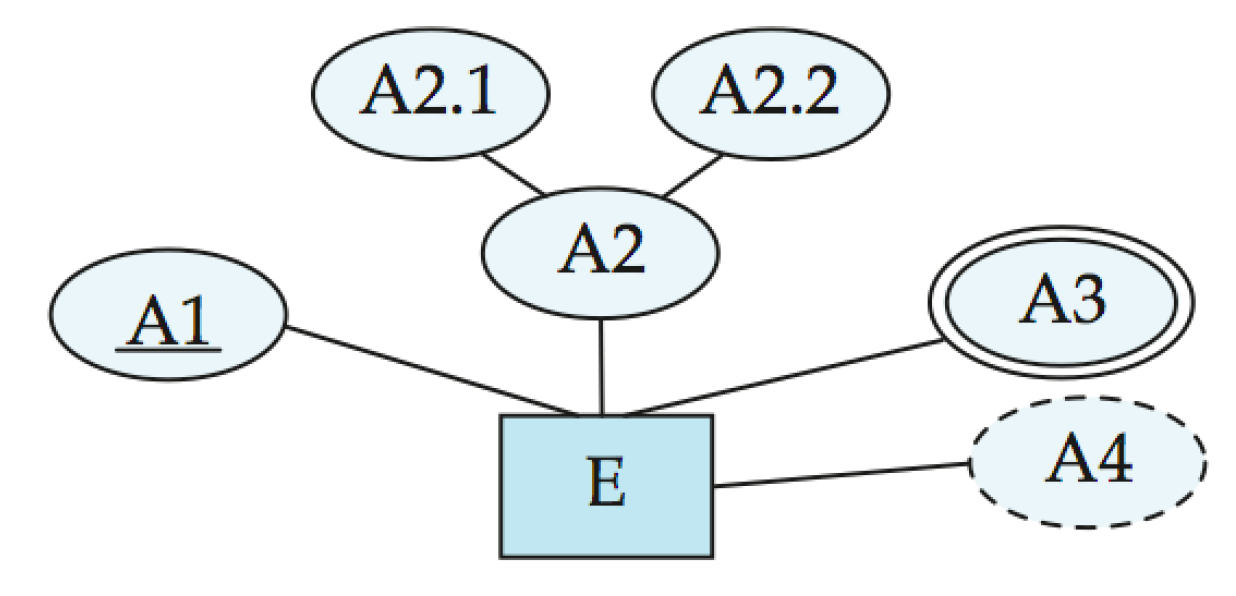
\includegraphics[width=6cm, height=4cm]{./imagenes/entidad.png}
				\caption{Entidad de nombre E, Atributo simple A1, Atributo compuesto A2, Atributo multivalorado A3, Atributo derivado A4, Clave primaria A1}
			\end{figure}

	\section{Claves}
		\begin{itemize}
			\item Una \textbf{superclave} de un CE es un conjunto de uno o más atributos cuyos valores unívocamente determinan cada entidad.
			\item Una \textbf{clave candidata} de un CE es una superclave minimal (i.e. si se quita atributo dejamos de tener superclave).
			\item Una \textbf{clave primaria} es aquella seleccionada de entre todas las claves candidatas que puedan existir.
		\end{itemize}
		
	\section{Correspondencia de cardinales}
		\begin{itemize}
			\item \textbf{Conjuntos de relaciones uno-uno:} una entidad de \textbf{E1} está asociada con a lo más una entidad de \textbf{E2} vía una relación \textbf{R}. Una entidad de \textbf{E2} está asociada con a lo más una entidad de \textbf{E1} vía \textbf{R}.
			\item \textbf{Conjuntos de relaciones uno-varios / varios-uno:} una entidad de \textbf{E1} está asociada con ninguna o varias entidades de \textbf{E2} vía una relación \textbf{R}. Una entidad de \textbf{E2} está asociada con a lo más una entidad de \textbf{E1} vía \textbf{R}.
			\item \textbf{Conjuntos de relaciones varios-varios:} una entidad de \textbf{E1} está asociada con ninguna o varias entidades de \textbf{E2} vía \textbf{R}. Una entidad de \textbf{E2} está asociada con a lo más una entidad de \textbf{E1} vía \textbf{R}.
		\end{itemize}
		
		\begin{center}
			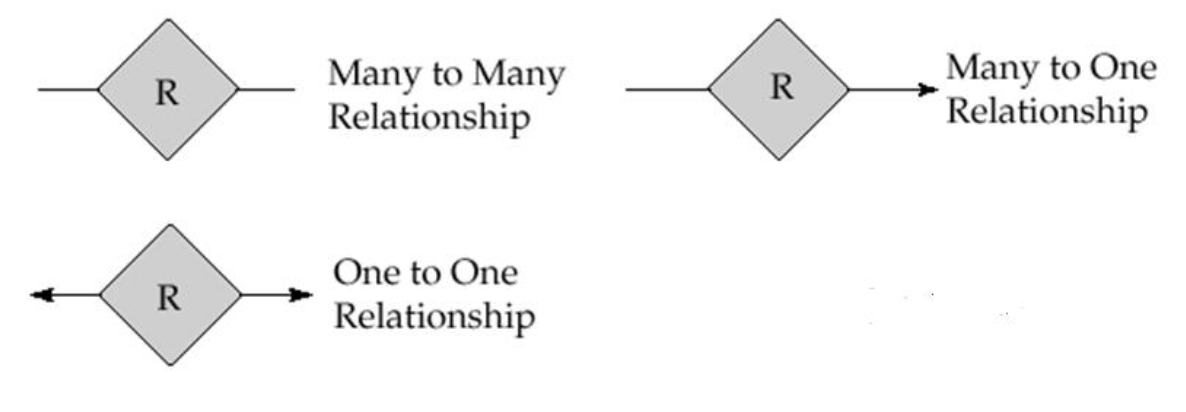
\includegraphics[width=10cm, height=4cm]{./imagenes/correspondencia.png}
		\end{center}
		
	\section{Formas de participación}
		\begin{itemize}
			\item \textbf{Participación total:} toda entidad en el conjunto de entidades participa en al menos una relación en el conjunto de relaciones. Es indicada por una línea doble.
			\par \underline{Ejemplo:} participación de caja de ahorro en cliente es total. Toda caja de ahorro debe tener clientes asociados.
			\item \textbf{Participación parcial:} algunas entidades no participan en alguna relación en el conjunto de relaciones.
			\par \underline{Ejemplo:} participación de instructor en supervisor es parcial.
		\end{itemize}
		
	\section{Conjunto de entidades débiles}
		Un CE que no tiene una clave primaria en el conjunto de sus atributos, se llama \textbf{conjunto de entidades débiles}. La existencia de un CE débiles depende de la existencia de un CE fuertes llamado \textbf{CE identificador}. 
		\vspace{5mm}
		\par \underline{Ejemplo:} ¿En el caso de libro-biblioteca cuál sería el CE identificador?
		\vspace{2.5mm}
		\par Hay un CR varios-uno entre CE débil y CE identificador, donde el CE débil tiene participación total, a este CR se le llama \textbf{CR de identificación}. El mismo se representa con un diamante doble.
		\par El \textbf{discriminador} de un CE débiles es un conjunto de atributos que permite distinguir entre todas las entidades de un CE débiles asociadas a la misma entidad fuerte. 
		\par Para identificar las entidades débiles se forma la clave primaria del CE con la clave primaria del CE identificador más el discriminador del CE débiles.
		
	\section{Diseño de una DB de calidad}
		\subsection{Eliminacion de información redundante}
			Una vez que se han decidido los CE del problema y los atributos de los CE se pasa a definir los CR, esos CR pueden señalar que algunos atributos en CEs son redundantes y por lo tanto necesitan ser removidos.
			
			\underline{Ejemplo:}
			\begin{itemize}
				\item CE \textbf{aula} con atributos (edificio, número y capacidad)
				\item CE \textbf{sección} con atributos (idCurso, idSec, semestre, año, edificio, número)
				\item CR \textbf{sec-aula} que relaciona secciones con aulas
				\end{itemize}
				
				\par ¿Qué pasa con esta propuesta?
				\begin{itemize}
				\item edificio y número aparecen en ambos CE pero son clave primaria de aula
				\item Luego edificio y número son redundantes en \textbf{sección} y deben ser removidos de allí
				\end{itemize}	

		\subsection{Uso de CE vs Atributos}
			A veces tenemos dos alternativas para modelar un objeto perteneciente a un CE E, como un CE o como un atributo de E.
			\begin{itemize}
				\item Cuando el CE E tiene un solo objeto que tiene un solo valor (atómico), conviene modelar al objeto como un atributo simple.
				\item Cuando el CE E tiene cero o más objetos que tienen un solo valor (atómico), se puede modelar al objeto como un atributo multivalorado.
				
				\item Cuando el objeto tiene varios atributos y es poseído por una sola entidad del CE E, conviene modelar el objeto como CE. La razón es que “ser poseído por una sola entidad” no se puede representar usando un atributo.
				\item Cuando el objeto tiene varios atributos algunos de los cuales no son de clave primaria del objeto y es poseído por varias entidades del CE E, conviene modelar el objeto como CE. La razón es que los atributos del objeto que no se usan para identificarlo generan redundancia de información, cosa que no pasa cuando el objeto se representa un como CE.
			\end{itemize}
			
		\subsection{Errores comunes}
			\par Un error muy común es usar la clave primaria de un CE como atributo de otro CE en lugar de usar un CR. La forma correcta sería usar un CR que vincule los dos CE, ya que hace la conexión entre los dos CE explícita, en lugar de implícita vía atributos de la clave primaria de uno de los CE.	
		
		\subsection{Uso de CEs vs uso de CR}
			\par Muchas veces son posibles dos alternativas para modelar un asunto, como un CE o como un CR.
			\begin{itemize}
				\item Si CR es uno-varios o varios-uno: si hay atributos, no de clave primaria en el CE A, entonces los atributos de A que no son de clave primaria dan lugar a redundancia de información si se usa alternativa CE. Por lo que conviene usar la opción CR en lugar de CE.
				\item Si el CR es varios – varios: si en al menos un CE hay atributos que no son de clave primaria, entonces ocurre igual que antes, los atributos del CE que no son de clave primaria dan lugar a redundancia de información si se usa la opción CE. Por lo que conviene usar CR en lugar de CE.
			\end{itemize}
		
		\subsection{CR de grado > 2 vs CR binarias}
			\par A veces tenemos las alternativas de modelar una situación como un CR de grado > 2 o como varios CR binarios. Si con los CR binarios puedo capturar los datos del CR de grado > 2 y puedo expresar más restricciones de integridad que con el CR de grado > 2, entonces usar los CR binarios.
		
		\subsection{CE débiles vs Atributo multivalorado compuesto}
			\par A veces para modelar una situación tenemos dos alternativas un CE débiles o un atributo multi-valorado compuesto. Si el objeto contemplado tiene su complejidad e involucra varios atributos y es de suma importancia para la organización, es poco conveniente tenerla como un atributo de un CE fuerte, por lo tanto, conviene modelarlo como un CE débiles.
			\par Si los objetos siendo considerados están relacionados con entidades de un CE fuerte que no es de identificación, entonces es necesario modelar dichos objetos como CE débiles.
		
	\section{Especialización - Generalización}
		Cuando en un diseño ER hay varios CE que son bastante similares en el sentido que comparten varios atributos en común, que tienen las mismas claves primarias y que participan en los mismos CR, aparecen problemas de repetición.		
		\par Esto es malo ya que estos modelos ocupan demasiado espacio. Muchos CR hacen el diagrama más intrincado, esto se ve agravado cuando el esquema de la BD tiene muchos CE y CR. Al cambiar un CE o CR muchas veces hay que propagar el cambio a otros CE o CRs.
		
		\par La solución a este problema es utilizar especialización-generalización.
		\begin{itemize}
			\item \textbf{Especialización:} hace referencia a un proceso de diseño \textit{top-down} donde designamos subgrupos dentro de un CE que son distintivos de otras entidades en el CE. Estos subgrupos son CE de más bajo nivel que tienen atributos específicos o participan de CR que no aplican al CE de más alto nivel. Una especialización se denota con un triángulo etiquetado ISA. La relación ISA se llama también relación de superclase – subclase.
			\item \textbf{Herencia de atributos:} un CE de más bajo nivel hereda:
				\begin{itemize}
					\item todos los atributos
					\item la clave primaria
					\item participaciones en CR del CE de más alto nivel con el cual está relacionado. 
				\end{itemize}
			\item \textbf{Generalización:} hace referencia a un proceso de diseño \textit{bottom up} que generaliza unos cuantos CE que comparten las mismas propiedades en un CE de más alto nivel.
			
			\vspace{7mm}
			\textbf{Restricciones de integridad:}
           \par Para indicar si una entidad pertenece o no a más de un CE de nivel más bajo dentro de la generalización.
         		\begin{itemize}
         			\item \underline{Disjunto:} una entidad puede pertenecer a solo un CE de nivel más bajo. Usar palabra reservada \textit{disj}.
					\item \underline{Solapado:} una entidad puede pertenecer a más de un CE de nivel más bajo.
				\end{itemize}         		  

			\vspace{7mm}			
			\textbf{Restricciones de completitud:} 
			\par Para indicar si una entidad en el CE de nivel más alto debe pertenecer a al menos uno de los CE de nivel más bajo en la generalización.
				\begin{itemize}
					\item \underline{Total:} una entidad debe pertenecer a un CE de nivel más bajo. Usar línea doble.
					\item \underline{Parcial:} una entidad puede no pertenecer a un CE de nivel más bajo.
				\end{itemize}
		\end{itemize}

	\section{Esquemas e instancias relacionales}
		\underline{Definiciones:}
		\begin{itemize}
			\item A1, A2, …, An son \textbf{atributos}
		 	\item R = (A1, A2, …, An ) es un \textbf{esquema de relación}
		 
		 	\par Dado un enunciado en lenguaje natural, se puede identificar atributos primero, y luego se pueden proponer esquemas de relación para distintos conceptos del problema actual.
			\item Dados conjuntos $D_{1}, D_{2}, \dotsc D_{n}$ una \textbf{relación r} es un subconjunto de $D_{1}, D_{2}, \dotsc D_{n}$. Las relaciones son conjuntos (el orden entre las tuplas no importa).
			\item Se puede pensar una relación como una tabla con columnas para los dominios $D_{1}, D_{2}, \dotsc D_{n}$ respectivamente.
			\item Un \textbf{elemento} \textit{t} $\in$ r es una tupla representado mediante una fila de la tabla.
		\end{itemize}
			\par Notar que el concepto de relación en el modelo relacional no tiene nada que ver con el concepto de relación en el modelo ER. Es más bien como están acostumbrados a trabajar en matemática.
			\par Se puede expresar la información manejada por una organización como un conjunto de relaciones o tablas, en cada columna se deciden los dominios con los que se trabaja para los valores.
			
			\vspace{5mm}
			\par \underline{\textbf{Notación:}} r(R) significa r es una relación con esquema de relación R, es decir, las columnas de r tienen como nombres los atributos de R.
			\begin{itemize}
				\item Los conceptos del problema que se asociaban a esquemas de relación ahora se terminan asociando también a relaciones o tablas de la BD.
				\item Los dominios de las tablas pasan a ser los dominios de los atributos del esquema relacional.
				\item Además es más fácil de comprender una tabla donde las columnas tienen los nombres de un esquema de relación.
			\end{itemize}

	\section{Tipos de atributos}
		\par El conjunto de valores permitidos para cada atributo se llama \textbf{dominio del atributo}. Se requiere que los valores de los atributos sean atómicos; esto es, indivisibles.

		\par A veces no sabemos el valor de un atributo o el mismo aún no existe, para poder reflejar esto en la base de datos se utiliza el valor especial \textbf{null}, el cual es un miembro de todo dominio y significa que el valor es desconocido o no existe. Si para una tupla no tenemos el valor de un atributo por algun motivo, podemos poner null como valor para ese atributo.
	
	\section{DB relacionales}
		\underline{Definiciones:}
		\begin{itemize}
			\item Un \textbf{esquema de una BD relacional} es un conjunto de esquemas de relación $R_{1}, R_{2} \dotsc R_{n}$
R1,…,Rn
			\item \textbf{Una base de datos relacional} consiste de múltiples relaciones $r_{1}(R_{1}), r_{n}(R_{2}) \dotsc r_{n}(R_{n})$
			\par Primero definimos los conceptos del problema mediante esquemas de relación, luego definimos los datos como tablas asociadas a esos esquemas, por último podemos poblar las tablas, consultarlas y alterarlas.
			\item nombre de relación, expresado en minúscula, r, s, u, r1, r2, ….
			\item nombre de esquema de relación, expresado en mayúscula R, S, U, R1, R2, …
			\item sea t $\in$ r , r(R), A $\in$ R . t[A] es el valor de t en A.
			\item ea t $\in$ r , r(R). t[i] es el valor de t en atributo i-ésimo de R.
		\end{itemize}

		\subsection{Superclaves}
			\underline{Definición:} Sea K $\in$ R , R esquema de relación; K es una \textbf{superclave} de R si los valores para K son suficientes para identificar una tupla única en cada posible relación r(R). Observar que se habla de relaciones para el problema o situación del mundo real que está siendo considerando.
		
		\subsection{Claves candidatas y primarias}
			\par Una superclave K es una \textbf{clave candidata} si K es minimal, es decir, para todo atributo de K si se lo quito dejo de tener una superclave.
			\par No confundir clave candidata con superclave de cardinalidad mínima. Una de las claves candidatas es elegida para ser la clave primaria.
			\vspace{5mm}
			\par \underline{Notación:} Se indican los atributos de una clave primaria para un esquema de relación R subrayando los atributos de R que forman la clave primaria.

		\subsection{Claves foráneas}
			\par Sea $R_{1}$ una \textbf{relación referenciante} y $R_{2}$ una \textbf{relación referenciada}, entonces
			\begin{itemize}
				\item \underline{Restricción de clave foránea:} Los valores de uno o más atributos en una tupla de $R_{1}$ aparecen en uno o más atributos de una tupla en $R_{2}$.
				\item Los atributos referenciados en $R_{1}$ suelen formar una clave primaria del esquema de $R_{2}$.
				\item Los atributos referenciados de l$R_{1}$ suelen formar una clave candidata del esquema de $R_{2}$.
				
				\vspace{5mm}
				\textbf{Representación gráfica:}
				\item Los esquemas se representan con rectángulos conteniendo nombre de esquema y nombres de atributos.
				\item Los atributos de clave primaria se subrayan.
				\item Las restricciones de clave foránea se representan mediante flechas que van de atributos referenciantes (de esquema referenciante) a atributos referenciados (de esquema referenciado).
			\end{itemize}

	\section{Diseño de una DB relacional}
		\par Existen dos formas de diseñar una buena base de datos:
		\begin{itemize}
			\item Aprovechar un buen diseño de esquema ER: si se tiene un buen diseño de ER, se lo puede transicionar a un buen diseño relacional. 
			\item Obtener un buen diseño relacional a partir de los atributos y las restricciones de integridad del problema. La \textbf{teoría de normalización} trabaja con esta idea y trata con cómo diseñar buenos esquemas de BD relacionales.
		\end{itemize}
	
	\section{Reducción a esquemas relacionales}
		\par Se tiene un buen diseño de esquema de BD usando modelado-ER y se va a 
traducir a un conjunto esquemas relacionales con claves primarias y restricciones de clave foránea. Hay reglas de traducción que suelen resolver un porcentaje alto del problema pero esas reglas no contemplan todos los casos.

		\par Una propiedad de la traducción de diagramas ER a tablas que se debe respetar es que para cada CE y CR hay un esquema relacional único al cual se asigna el CE / CR.
		
		\vspace{5mm}		
		\par Además de los equemas de relación obtenidos por la traducción automática se debe obtener:
		\begin{itemize}
			\item Claves primarias de esquemas de relación: para esto se usa la información de claves primarias de CE.
			\item Restricciones de clave foránea: para esto se usa el tipo de elemento de modelo ER a mapear (p.ej. CR, CE débiles, atributo multivalorado, etc.).
		\end{itemize}

		\subsection{Regla CEF1}
			\par Un CE fuerte que no involucra atributos compuestos ni atributos multivalorados se mapea a un esquema relacional con los mismos atributos. La clave primaria del CE se convierte en la clave primaria del esquema relacional.

			\begin{center}
				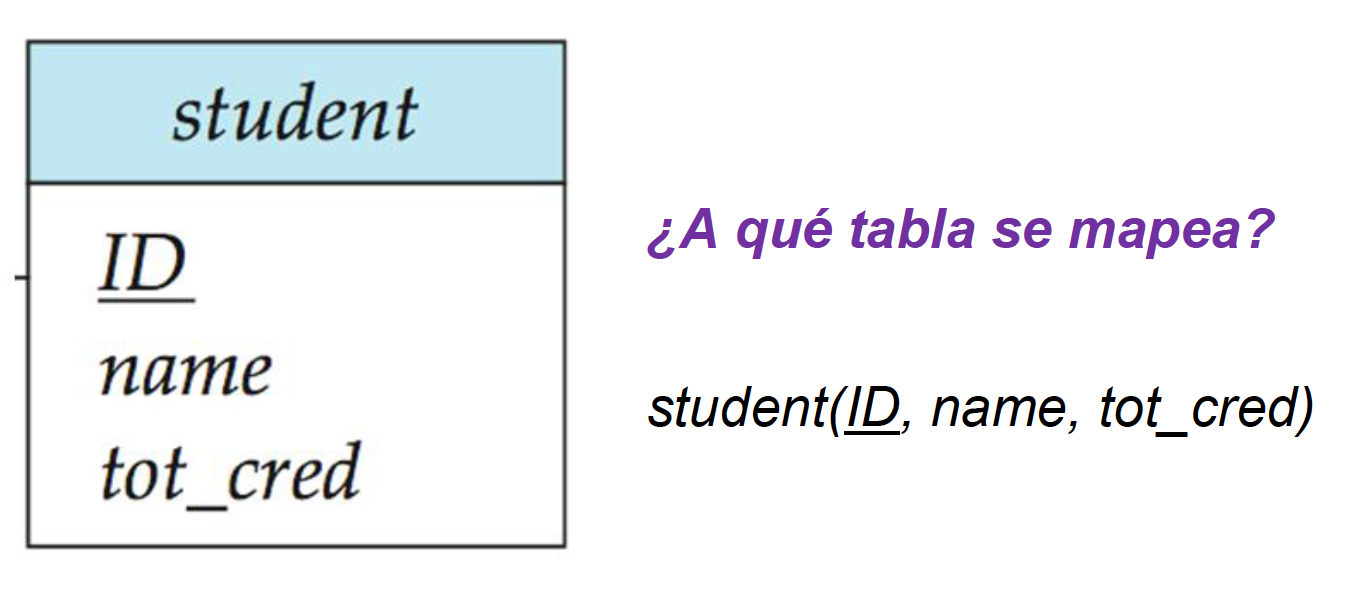
\includegraphics[width=7cm, height=3cm]{./imagenes/cef1.png}
			\end{center}
		
		\subsection{Regla CEF2}
			\par Un CE fuerte que no involucra atributos/subatributos multivalorados se mapea a un esquema relacional con los mismos atributos simples y los subatributos hoja de los atributos compuestos.
		
			\begin{center}
				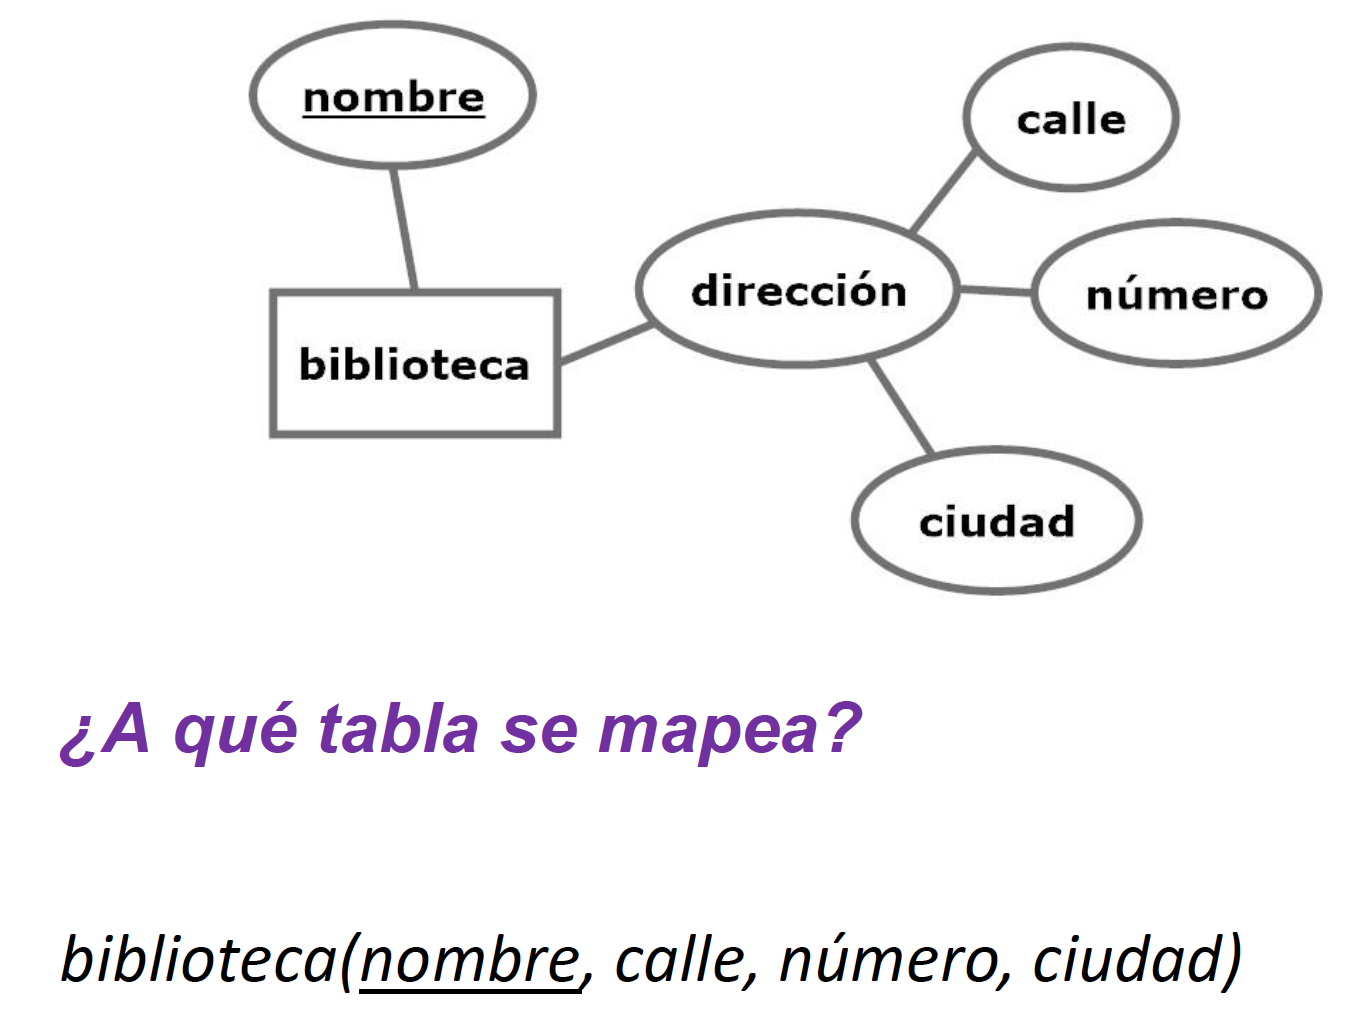
\includegraphics[width=9cm, height=5cm]{./imagenes/cef2.png}
			\end{center}
		
		\subsection{Regla CEF3}
			\par Un atributo multivalorado M simple de un CE E es representado por un esquema separado EM. EM tiene atributos correspondientes a la clave primaria de E y un atributo correspondiente al atributo multivalorado M. Todos los atributos de EM forman su clave primaria. Se pone una restricción de clave foránea desde EM que referencia a la clave primaria de E.
			
			\begin{center}
				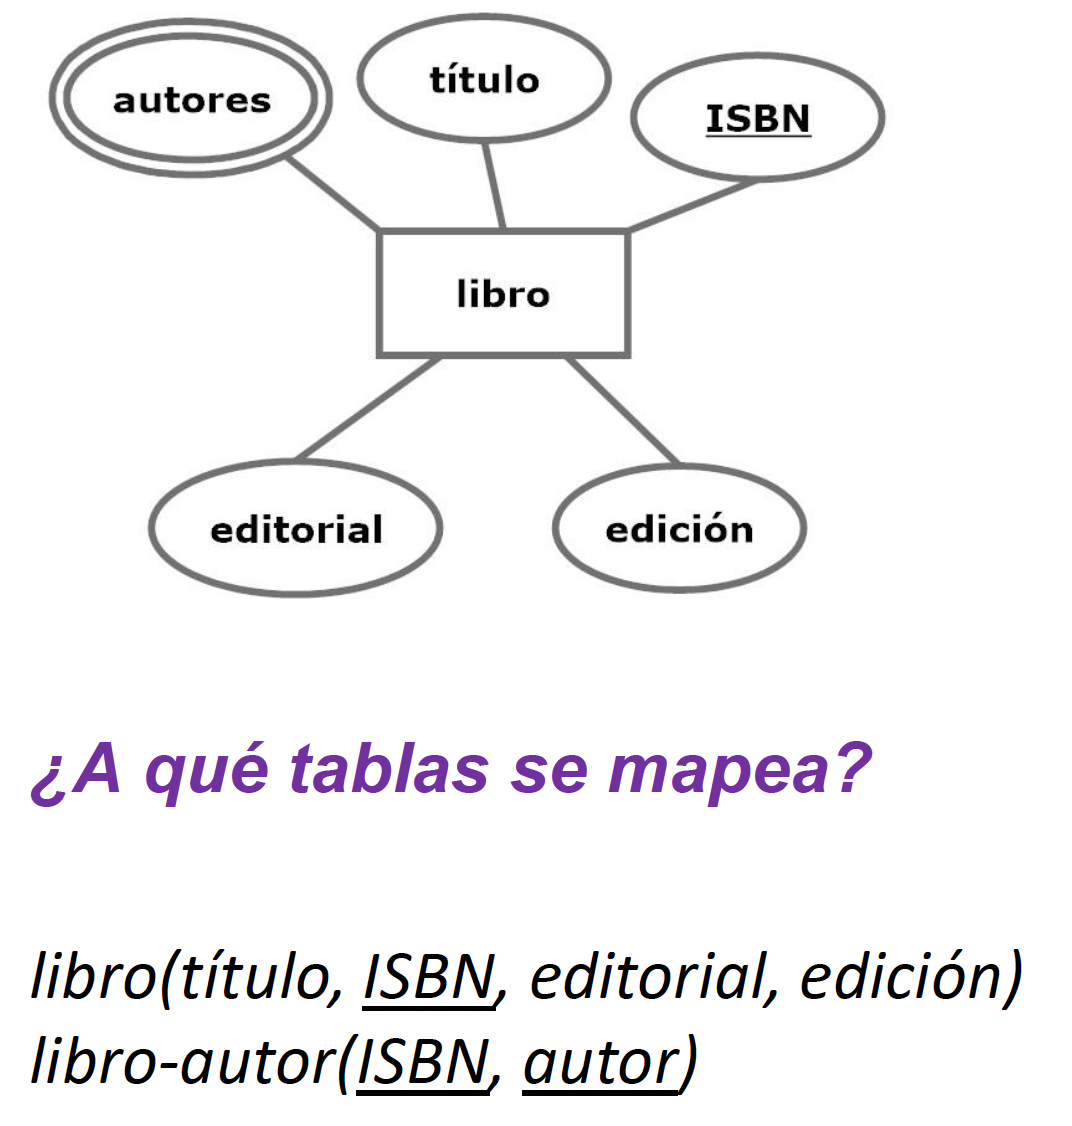
\includegraphics[width=8cm, height=7cm]{./imagenes/cef3.png}
			\end{center}
			
		\underline{\textbf{Aclaración:}} Cada valor del atributo multivalorado mapea a una tupla separada en la tabla del esquema EM.
		\par Por ejemplo un libro con ISBN 970-17-0256-5 y autores con DNIs: 11122256 y 15345678 se mapea a dos tuplas: (970-17-0256-5, 11122256 ) y (970-17-0256-5, 15345678)

		\vspace{7mm}
		\underline{\textbf{Decisión:}} Los atributos derivados no son explícitamente representados en el modelo de datos relacional. Se verá que si se los necesita una forma de computarlos es por medio de consultas.
		
		\subsection{Regla CR1}
			\par Un CR \textbf{varios a varios} es representado con un esquema con atributos para las claves primarias de los dos CE participantes y todos los atributos descriptivos del CR (que no son multivalorados). La clave primaria del esquema del CR es la unión de las claves primarias de los CEs que participan en el CR. Para cada CE que participa en el CR se crea restricción de clave foránea que referencia clave primaria de CE.

			\begin{center}
				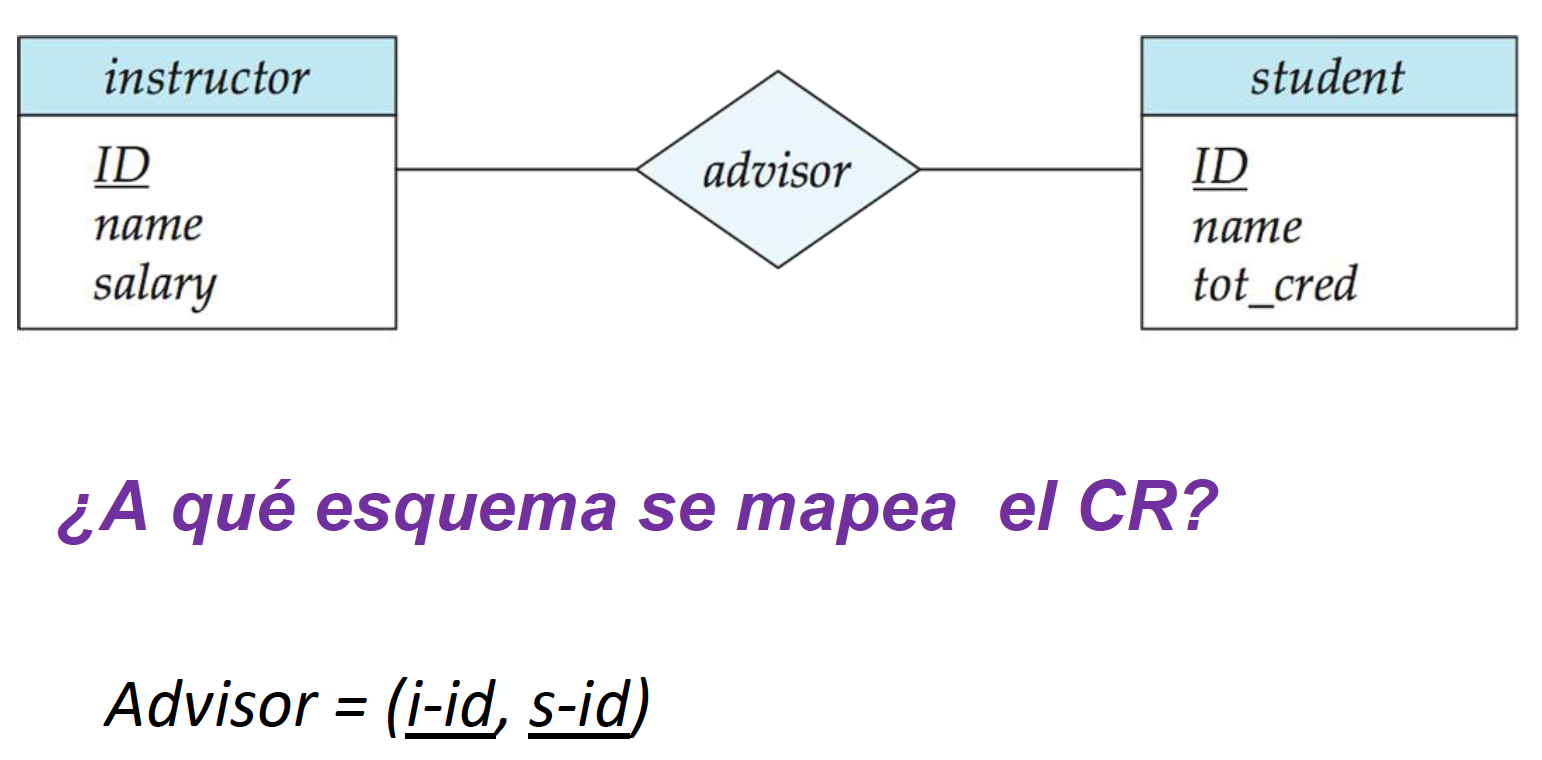
\includegraphics[width=8cm, height=5cm]{./imagenes/cr1.png}
			\end{center}

		\subsection{Regla CR2}
			\par Un CR \textbf{varios a uno} o \textbf{uno a varios} que es total en el lado varios puede ser representado agregando atributos extra en el CE del lado varios, conteniendo la clave primaria del lado uno. La clave primaria del CR es la clave primaria del CE del lado varios. Se crea restricción de clave foránea de CR que referencia a clave primaria de CE de lado varios.

			\begin{center}
				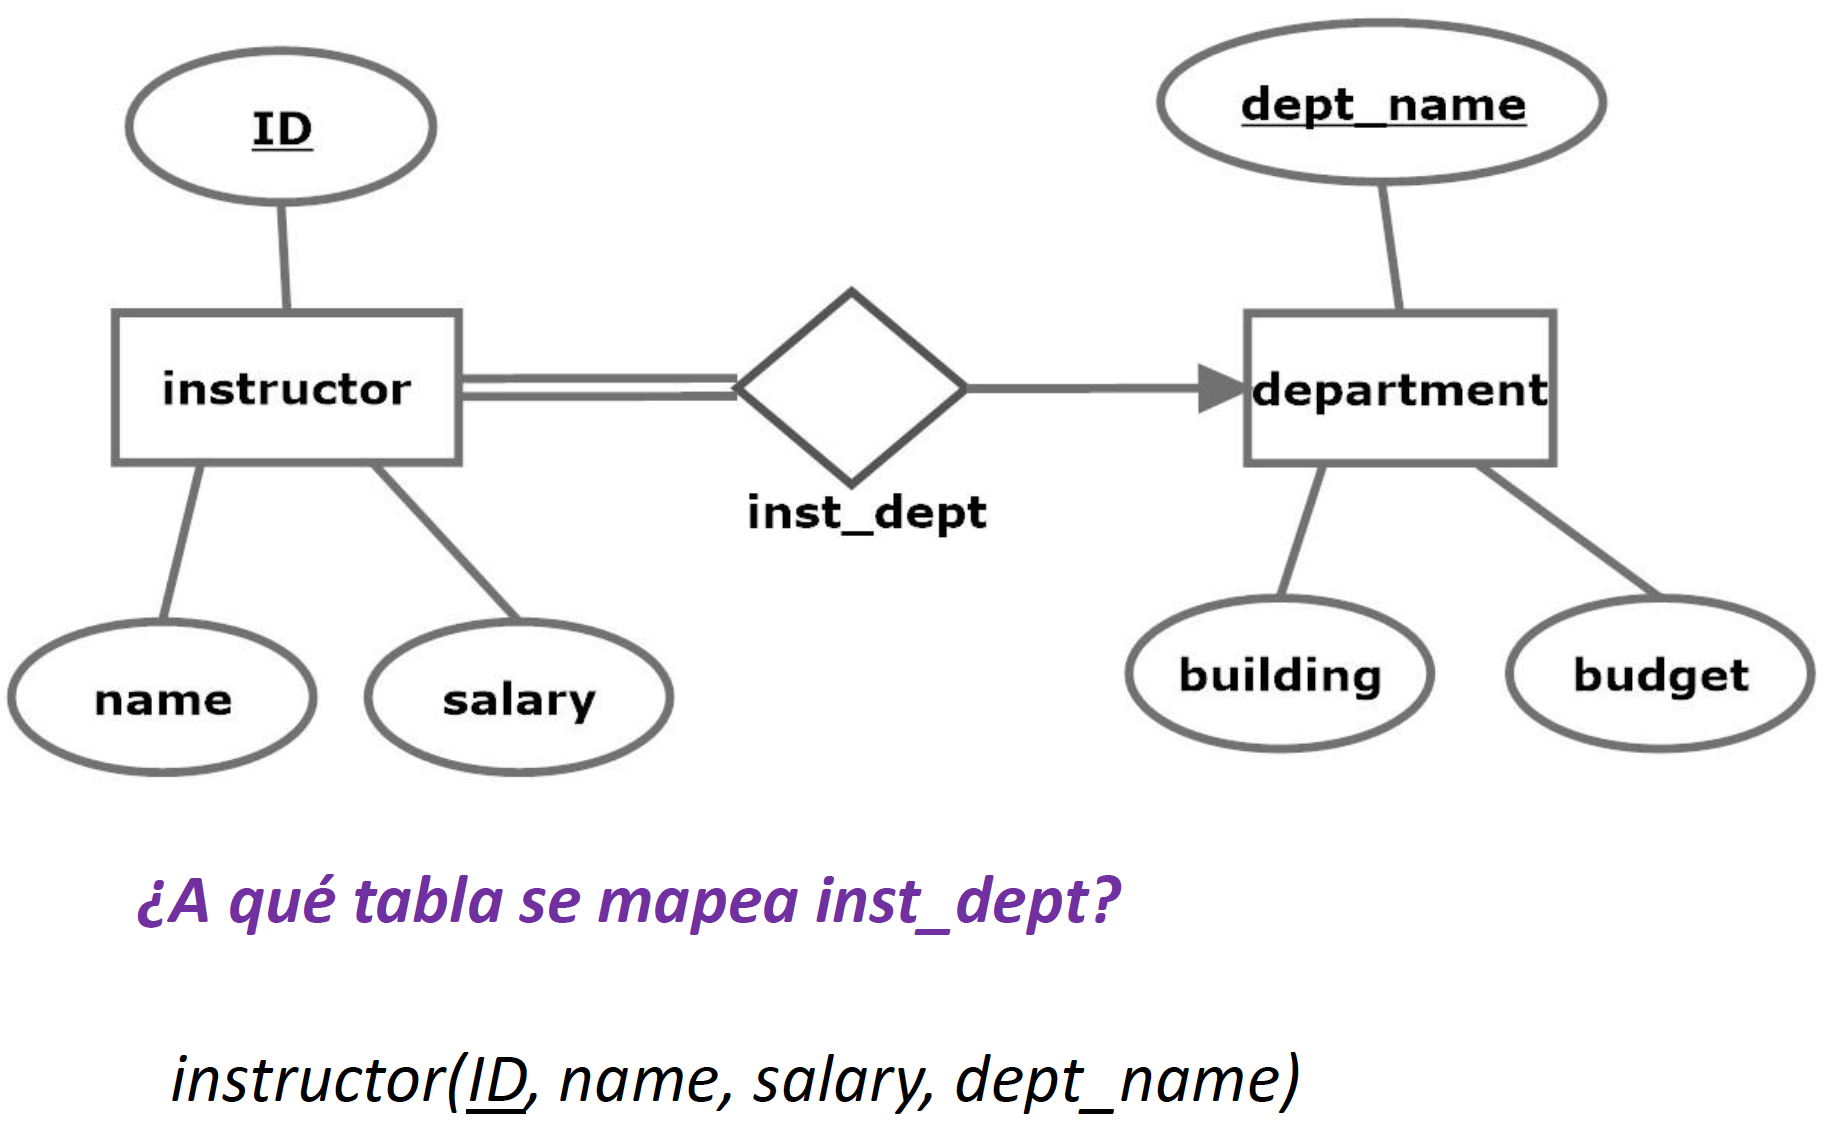
\includegraphics[width=7cm, height=5cm]{./imagenes/cr2.png}
			\end{center}

			\par Si la participación es parcial en el lado varios, aplicar la regla anterior puede resultar en valores nulos. Esto sucede cuando a una entidad del CE del lado varios no le corresponde ninguna entidad del CE del lado uno.
		
		\subsection{Regla CR3}
			\par Un CR \textbf{uno a uno} puede ser mapeado agregando al esquema resultante de traducir uno de los CE participantes los atributos de la clave primaria del otro CE. La clave primaria de cualquier CE puede ser elegida como la clave primaria del CR. Se crea restricción de clave foránea de esquema relacional asociado al CR que referencia clave primaria de otro CE (el que no se tomo de base para hallar el esquema asociado al CR).

			\begin{center}
				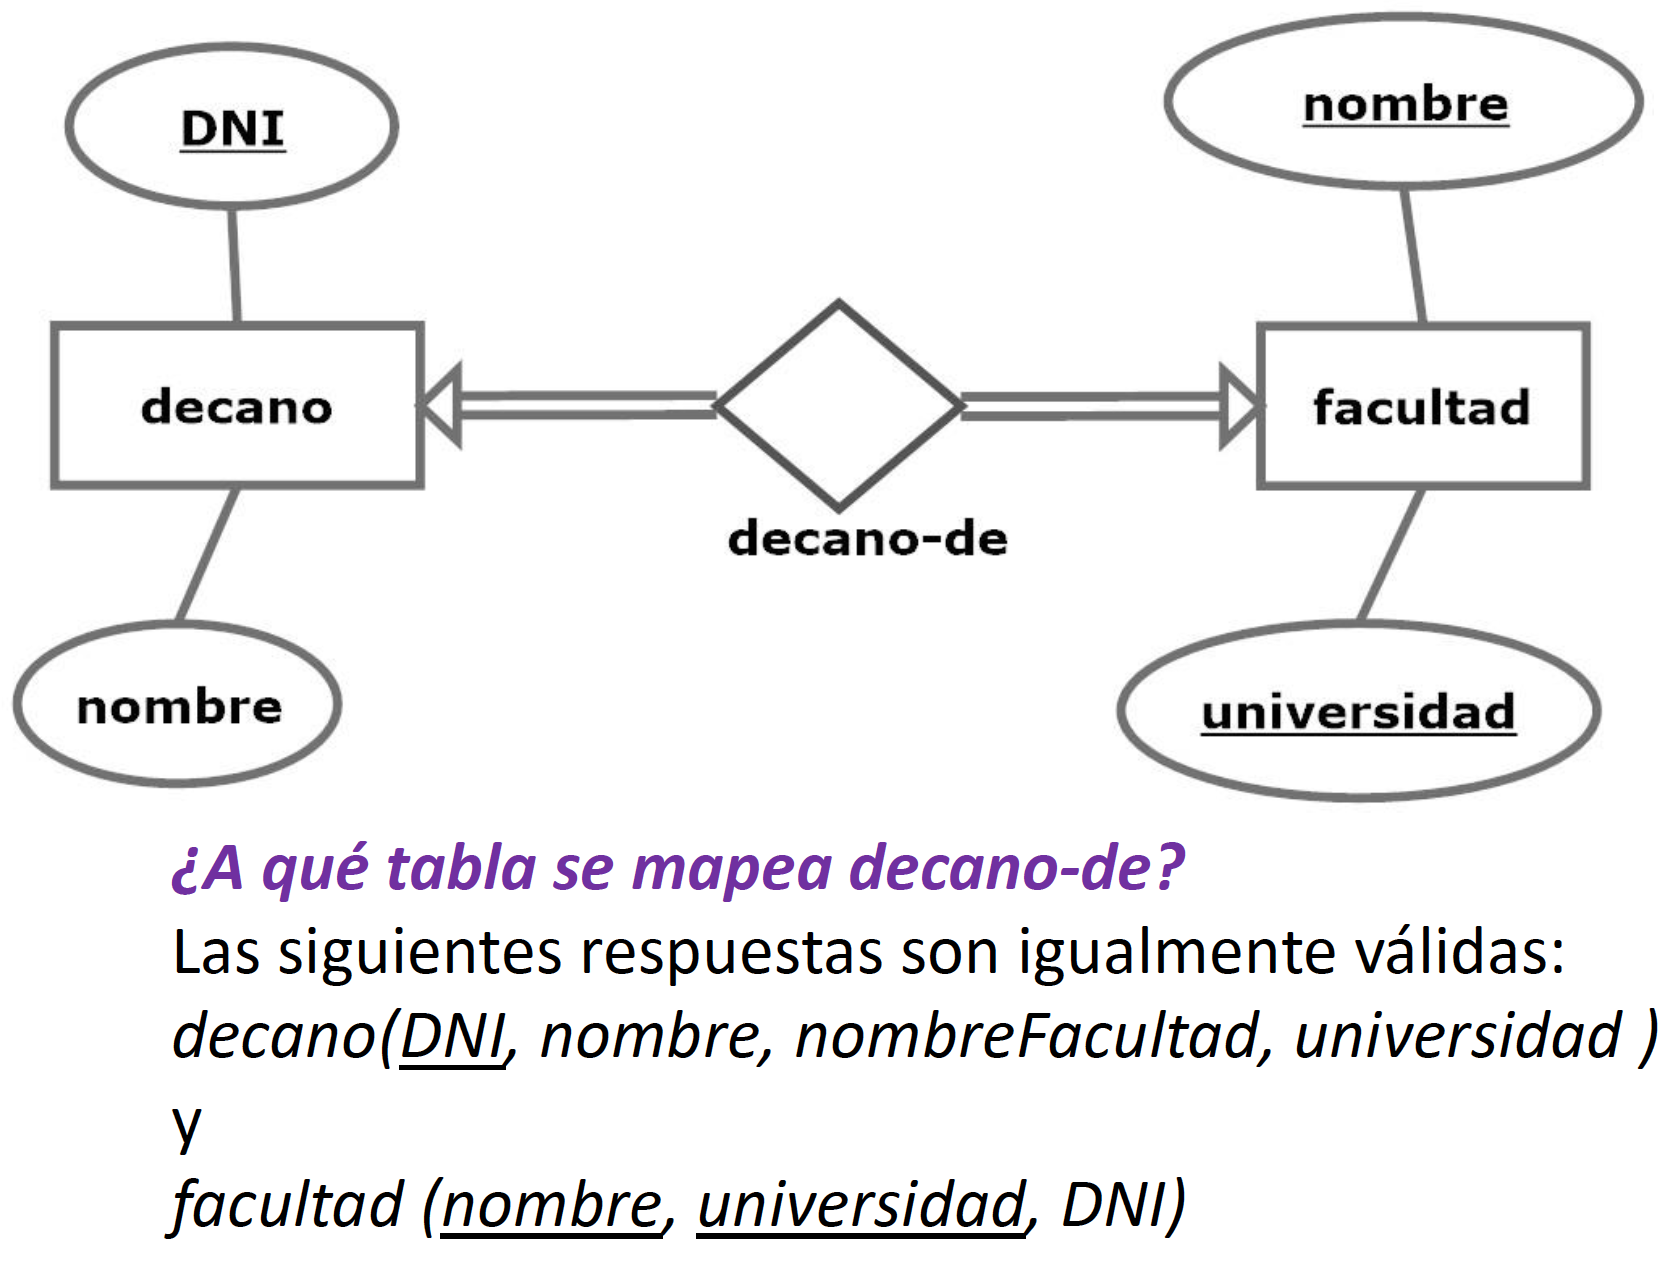
\includegraphics[width=6cm, height=5cm]{./imagenes/cr3.png}
			\end{center}

		\subsection{Regla CED}
			\par Un CE débiles se mapea a una tabla que incluye columnas para la clave primaria del CE identificador más los atributos (no multi-valorados) del CE débiles (achatando jerarquías de atributos compuestos si es necesario). La clave primaria del CE identificador más el discriminador del CE débil forman la clave primaria del esquema relacional de la traducción. Para atributos de esquema de CE débil que provienen de CE identificadora se agrega restricción de clave foránea desde esquema de CE débil a CE identificador. El CR identificador no se mapea.

			\begin{center}
				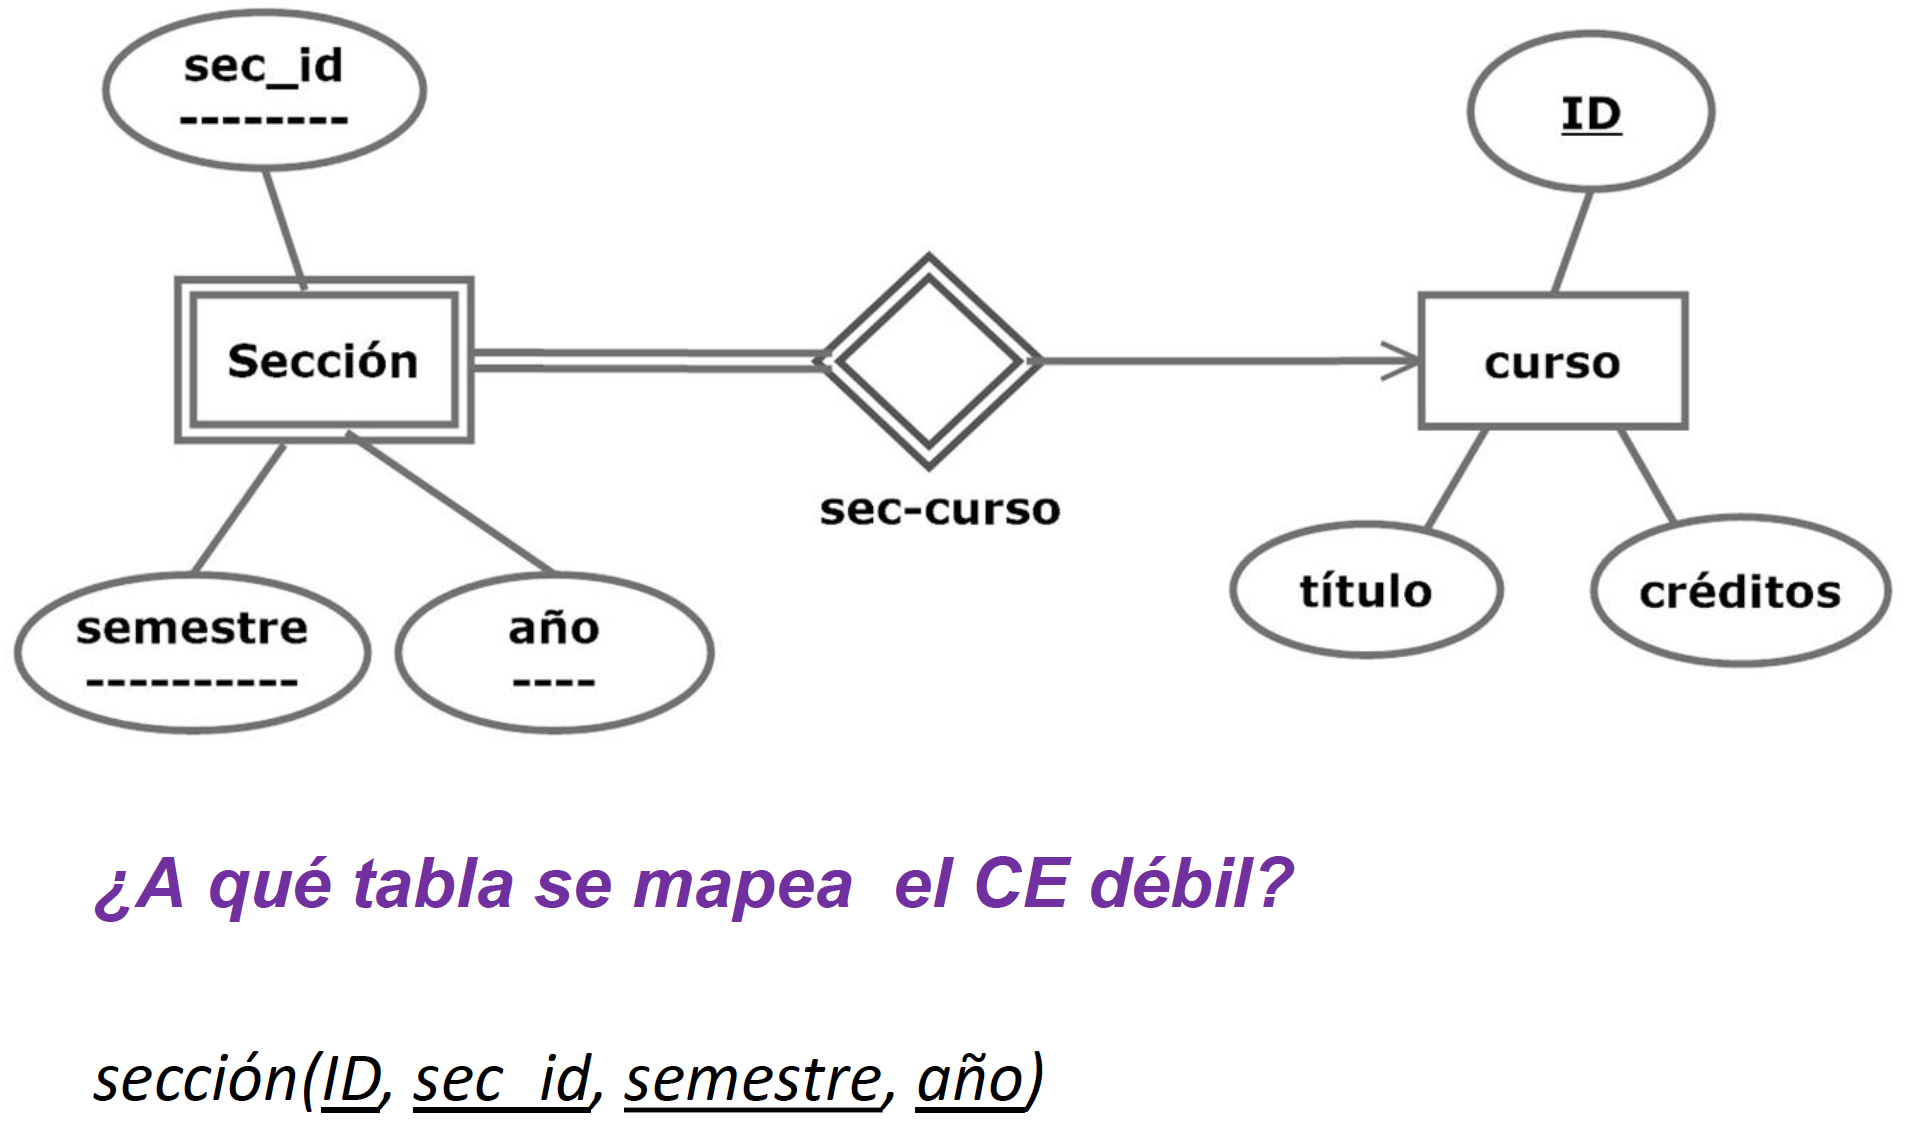
\includegraphics[width=7cm, height=5cm]{./imagenes/ced.png}
			\end{center}
			
		\subsection{Reducción de generalización}
			\par Para traducir generalización iremos proponiendo y evaluando ideas de traducción. Al final decimos bajo qué circunstancias las ideas de traducción son reglas a usar.
			
			\subsubsection{Idea G1:} traducción de generalización a tablas.
				\begin{itemize}
					\item Formar una tabla para el CE de nivel más alto (la generalización)
					\item Formar una tabla para cada CE especialización que incluye la clave primaria del CE generalización y los atributos locales.
				\end{itemize}

				\begin{center}
					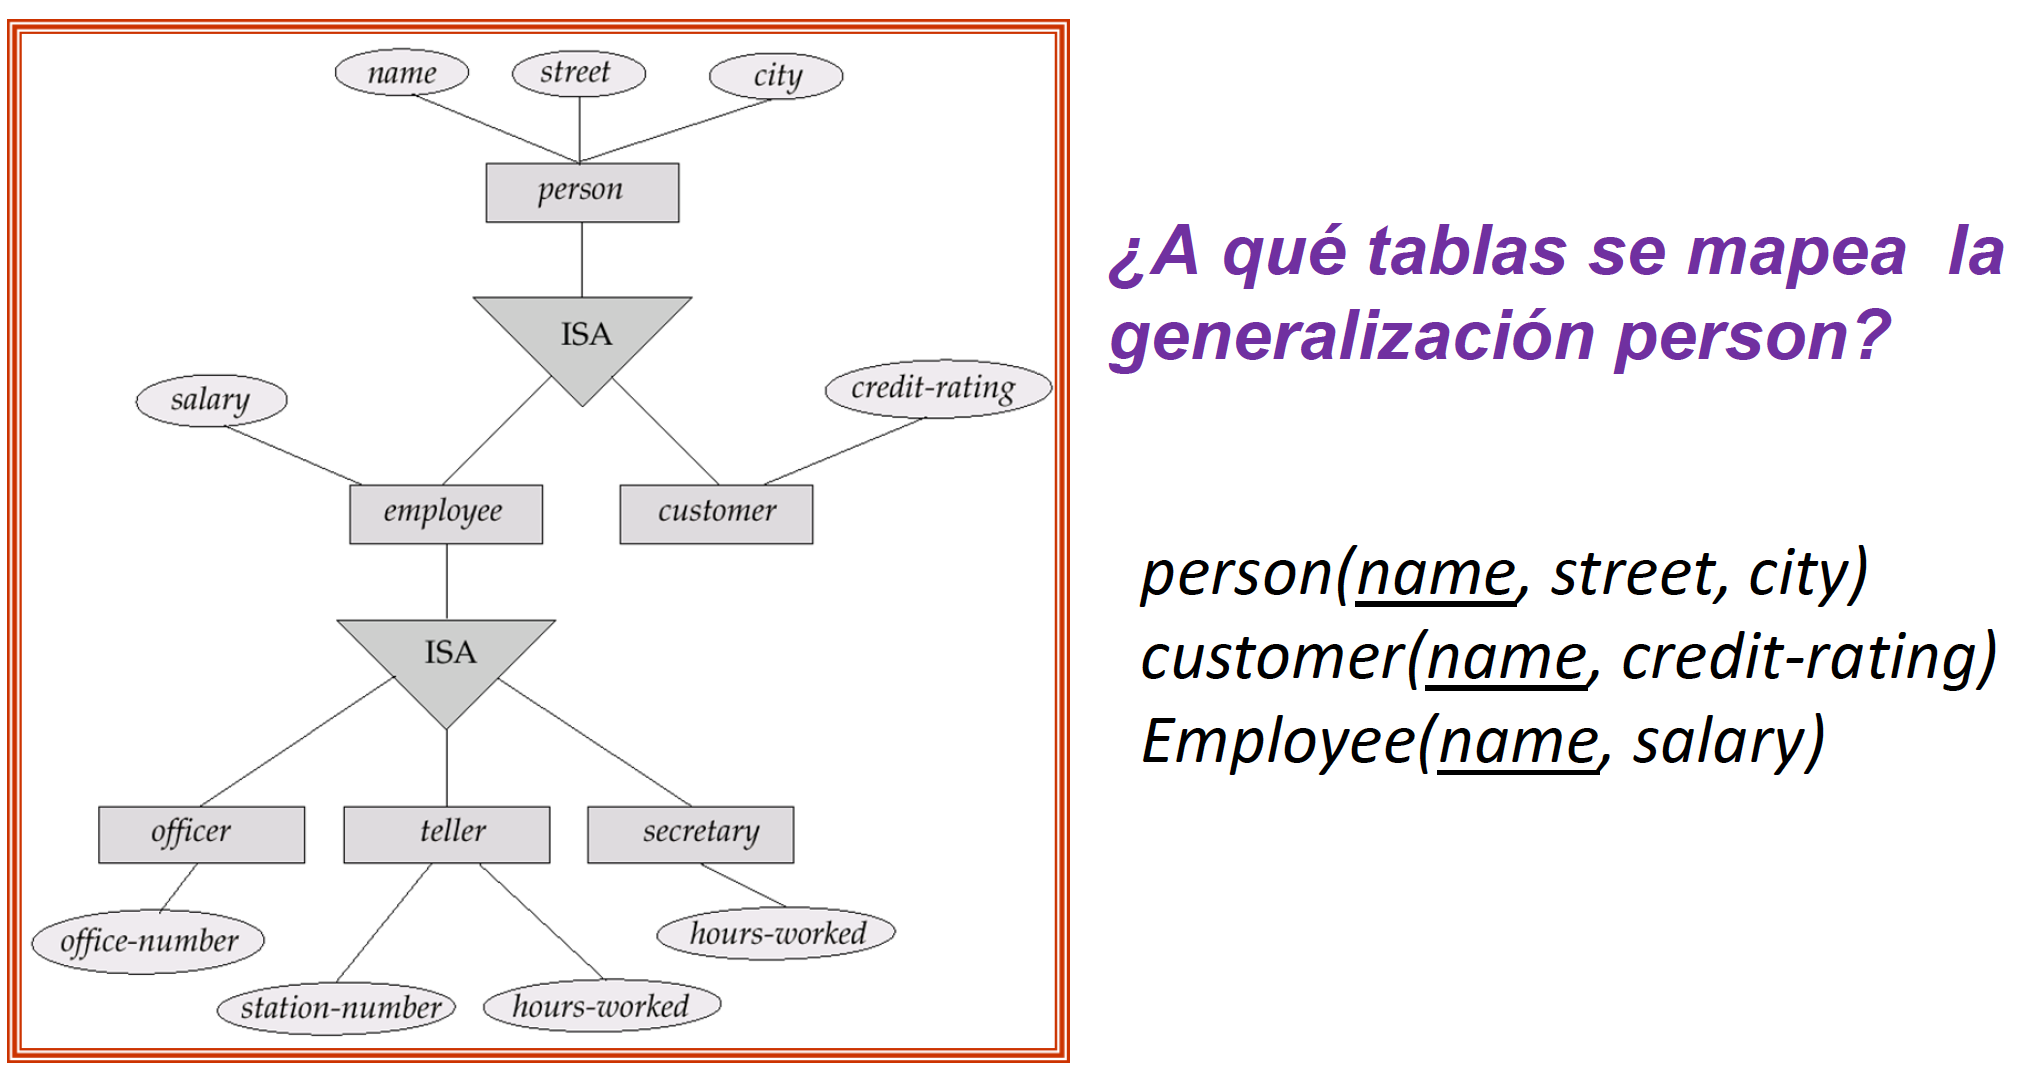
\includegraphics[width=11cm, height=7cm]{./imagenes/g1.png}
				\end{center}
			
				\underline{Evaluación de Idea G1:} obtener toda la información de CE de especialización requiere acceder a dos tablas.
			
			\subsubsection{Idea G2:} formar una tabla para cada CE especialización con los atributos locales y heredados del CE generalización.
			
				\begin{center}
					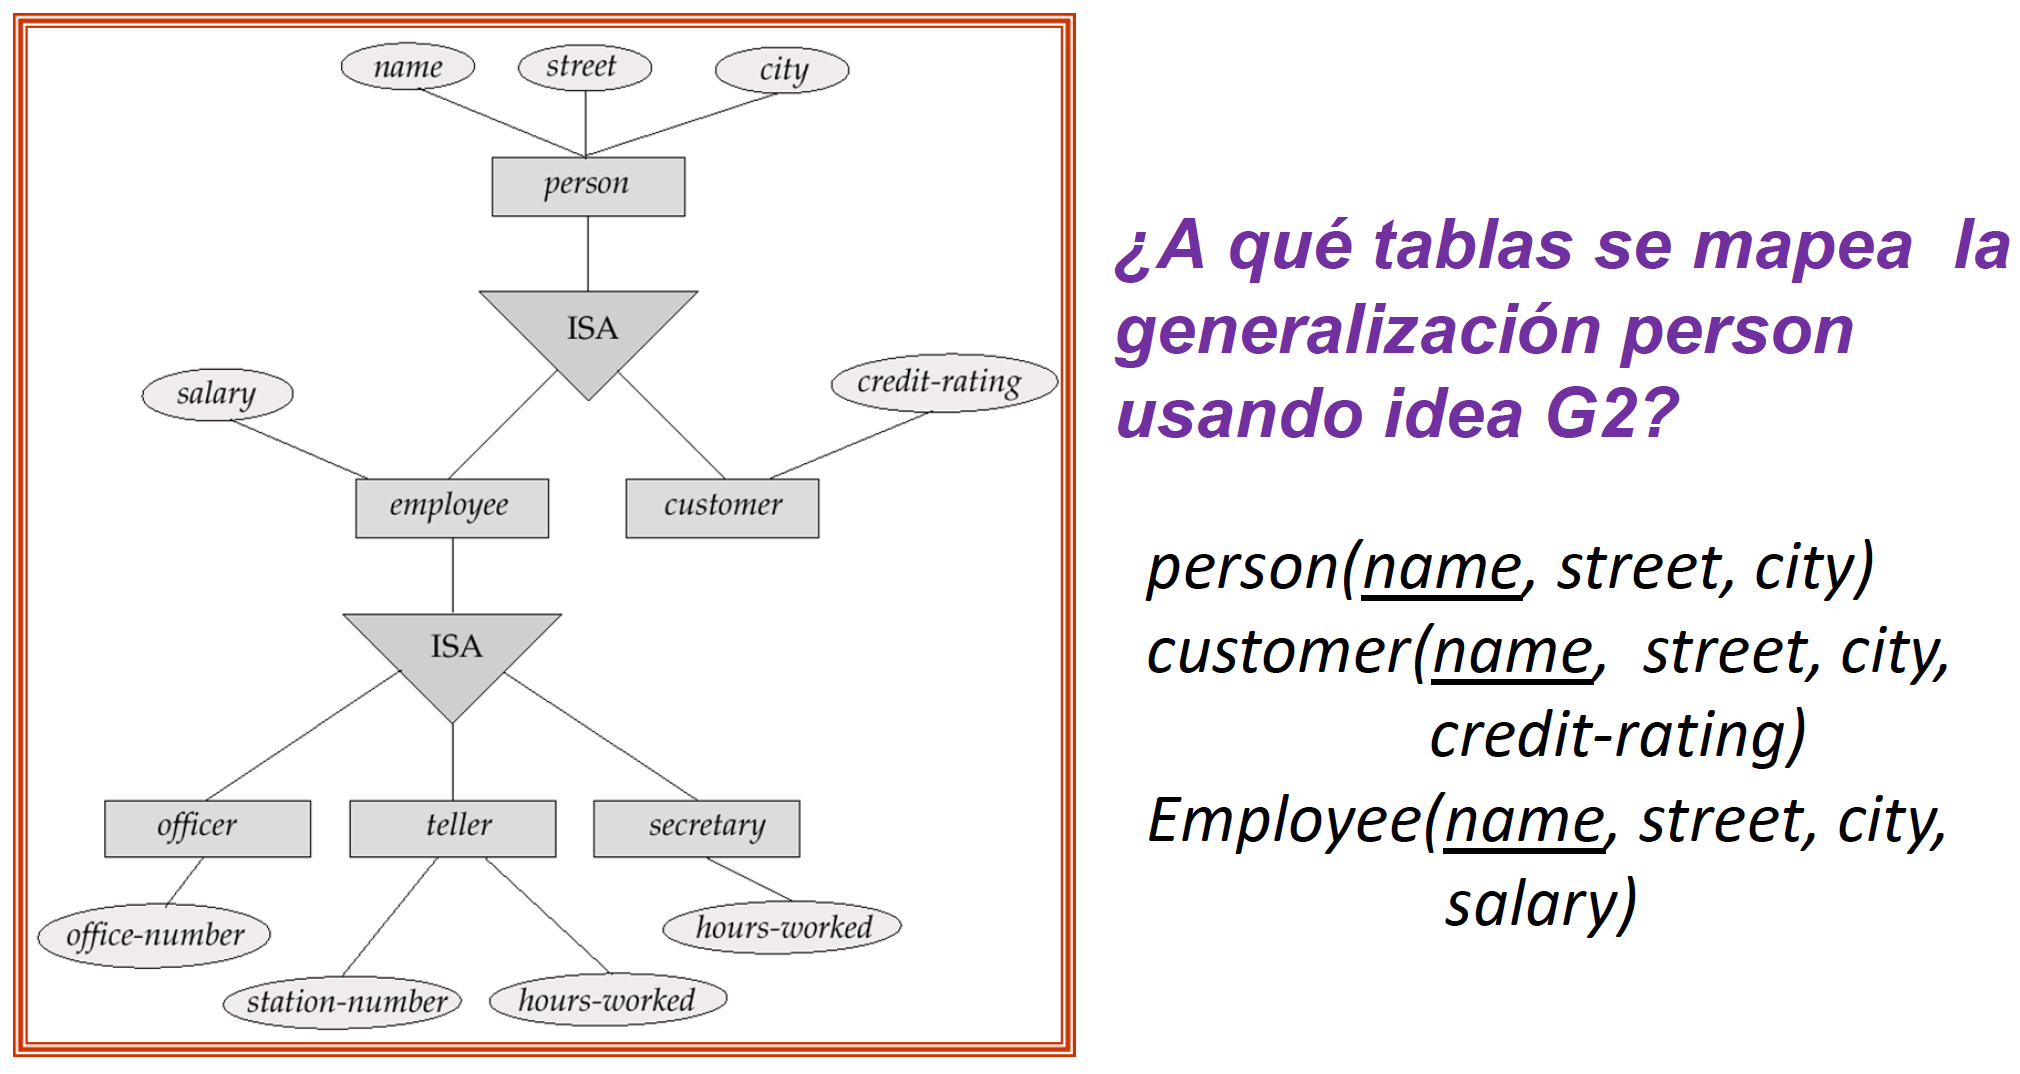
\includegraphics[width=11cm, height=7cm]{./imagenes/g2.png}
				\end{center}
			
				\underline{Evaluación de Idea G2:} si dos o más especializaciones contienen la misma entidad, entonces los atributos que no son clave primaria del CE generalización son almacenados redundantemente.
				
				\par Si la generalización es total con la traducción usando esta idea, la tabla del CE generalización no se requiere para almacenar información.
			
			\subsubsection{Idea G3:} si la generalización es total formar una tabla para cada CE especialización con los atributos locales y heredados; no formar tabla para la generalización. Esta idea es óptima para cuando la generalización es total y disjunta.

			\vspace{7mm}
			\textbf{En resumen:}
			\begin{itemize}
				\item Generalización total y disjunta: usar idea G3.
				\item Generalización no total y disjunta: usar idea G2.
				\item Generalización no disjunta: usar idea G1 (para evitar tener que tratar con redundancia de información).
			\end{itemize}

			
\chapter{Algebra Relacional}
		
\end{document}